\section{The Pixel Cluster Counting (PCC) method}
\label{sec:pcc}
(describe cluster reconstruction, the module selection/veto, cluster counting per bx, per LS,..) \\

Pixel cluster counting (PCC)  method is an offline technique for the calculation of instantaneous luminosity $(L_{inst})$ for any LHC run period by counting the number of pixel clusters in the pixel detector (innermost segment of the CMS tracker) in a zero bias event which requires that only two bunches cross at the CMS interaction point. The mean number of pixel clusters can be expressed in terms of mean number of pixel clusters per proton-proton interaction and the number of proton-proton interaction per bunch crossing that is also called pileup (PU). \\

$<N_{cluster}>$ = $<N_{cluster/interaction}>$ (PU)  or (PU) = $\frac{<N_{cluster}>}{<N_{cluster/interaction}>}$ \\

The instantaneous luminosity per bunch crossing $L_{inst/bunch}$ is proportional to the number of proton-proton (pp) interactions per bunch crossing (pileup) and the proportionality constant is the ratio of  LHC orbit frequency f and the pp interaction cross section $\sigma_{interaction}(\sqrt{s})$ where s is the proton-proton collision center-of-mass energy \cite{CMS-PAS-LUM-12-001}. \\

$L_{inst/bunch}$ = $\frac{f}{\sigma_{interaction}}$ (PU)  \\

$L_{inst/bunch}$ = $\frac{<N_{cluster}> \: f }{<N_{cluster/interaction}> \: \sigma_{interaction}(\sqrt{s})}$ \\

The PCC visible cross section $\sigma_{vis}$ which is a calibration constant between pixel clusters rate and luminosity can be defined as \\

$\sigma_{vis}$ = $<N_{cluster/interaction}>$  $\sigma_{interaction}(\sqrt{s})$ \\

\newpage Thus, instantaneous luminosity per bunch crossing is given by \\

$L_{inst/bunch}$ = $\frac{<N_{cluster}> \: \sigma_{interaction}(\sqrt{s}) \: f }{ \:\sigma_{vis} \: \sigma_{interaction}(\sqrt{s})}$ \\

$L_{inst/bunch}$ = $\frac{<N_{cluster}> \:\: f}{\sigma_{vis}}$ \\

The PCC visible cross section $\sigma_{vis}$ is determined using van der meer scan method which is described in section 5. Cluster counting can be done over different time periods like 1 bunch crossing (25ns), 1 Lumi section (23.36s), 4 Lumi nibble (1.46s) and similarly instantaneous luminosity can be calculated over these time periods using PCC method. \\

Specific techniques are employed for the reconstruction of clusters in the pixel detector and all the reconstructed clusters are used for counting to calculate the instantaneous luminosity. Algorithm used for finding clusters check for pixels whose signal to noise ratio is more than 6 and then merge adjacent pixel. These algorithms estimates cluster position in two directions and cluster charge. A cluster is a set of adjacent pixels and only pixels above certain minimum value of charge are considered. Position of a cluster in X and Y directions are obtained by fitting X and Y projections to templates that are estimates for cluster shapes \cite{Chatrchyan:2014fea}.


\begin{figure}[H]
  \centering
  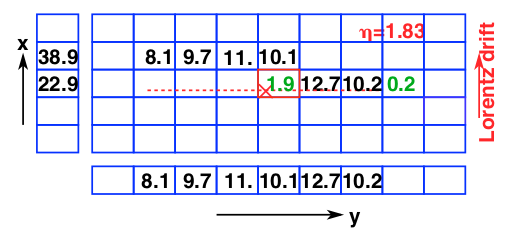
\includegraphics[width=0.6\columnwidth]{./pixel_reco.png}
  \caption{ \onehalfspacing Diagram showing pixel cluster with charge accumulation in each pixel expressed in terms of thousands of electrons. Green numbers represent charge accumulation below the 2000 electron threshold which are excluded clusters. The dotted red line indicates the particle trajectory projection in the module plane and the red cross shows the position of true hit.}
  \label{fig:CMS}
\end{figure}








